\chapter{Pr�paration d'un horaire avec DIAMANT}

Nous d�taillerons ici les �tapes n�cessaires � la construction d'un horaire (cycle et examen). Toutefois,
les options du logiciel ne seront pas toutes pr�sent�es. Certaines �tapes sont les m�mes tant pour les horaires de cours que ceux d'examen, tandis que d'autres sont diff�rentes.
On suppose que l'utilisateur a d�j� sur son ordinateur les fichiers n�cessaires (ceux du STI et
ceux de la Facult�) : cours.sig, choixet.sig, disprof.sig et locaux.txt. Ces fichiers peuvent porter
n'importe quel nom, mais pour notre exemple, les noms sont bien explicites. Il est n�cessaire de
regrouper toutes les informations concernant les horaires d'un trimestre dans un r�pertoire (par
exemple hiver04 ou h2004). Ainsi, les fichiers d'importation et les fichiers associ�s � un horaire
seront ensemble.

\section{Horaire de cycle}

On suppose aussi qu'il s'agit de la pr�paration d'un nouvel horaire.

\begin{enumerate}
    \item Lancer DIAMANT.
    \item Aller au menu \textbf{\emph{Fichier}}, puis selectionner le menu \textbf{\emph{Nouvel horaire}} et enfin selectionner le menu \textbf{\emph{Horaire cycle}}. Une bo�te de dialogue comme celle
de la Figure \ref{selectgrillecyc} doit appara�tre et elle vous permettra de choisir le fichier (fichier avec extension \emph{xml}) contenant la configuration de votre grille horaire.

\begin{figure}[h]
  % Requires \usepackage{graphicx}
  \begin{center}
    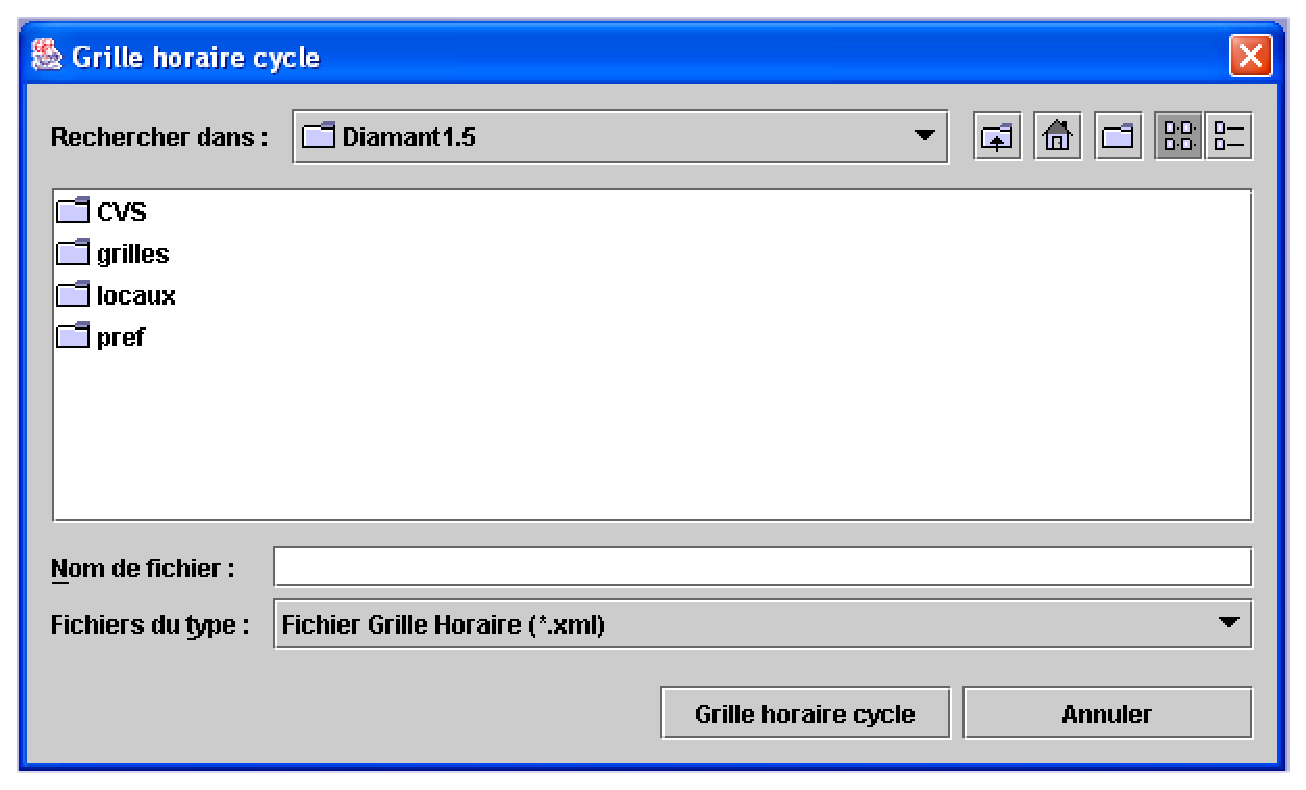
\includegraphics[width=3.5in]{UserManualInputs/images/selectXMLfile.eps}
    \caption{Selection de la grille horaire cycle}\label{selectgrillecyc}
  \end{center}
\end{figure}

    \item En cliquant sur le bouton \emph{\textbf{OK}}, la grille horaire s�lectionn�e est charg�e et pr�sent�e � l'�cran (voir figure \ref{grillecyc}).
\begin{figure}[h]
  % Requires \usepackage{graphicx}
  \begin{center}
    \includegraphics[width=4.5in]{UserManualInputs/images/grille.eps}
    \caption{Grille horaire cycle}\label{grillecyc}
  \end{center}
\end{figure}

    \item Aller au menu Fichier et s�lectionner le menu \textbf{\emph{D�finir fichiers � importer}}. Une bo�te de dialogue comme celle de la Figure \ref{defautoimport}  doit appara�tre. Rep�rer l'endroit o� chacun des fichiers est localis�, puis cliquer sur OK. Une nouvelle fen�tre se pr�sentera afin de vous permettre d'enregistrer la configuration (selection de fichiers) que vous venez de faire.  

Il est recommand� d'enregistrer cette configuration en utilisant un nom de fichier unique et repr�sentatif.

Exemple: choisissez le nom de fichier \emph{E02cours} pour \emph{�t� 2002 horaire de cours} et le fichier cr�� sera \emph{E02cours.dim}.

\begin{figure}[h]
  % Requires \usepackage{graphicx}
  \begin{center}
    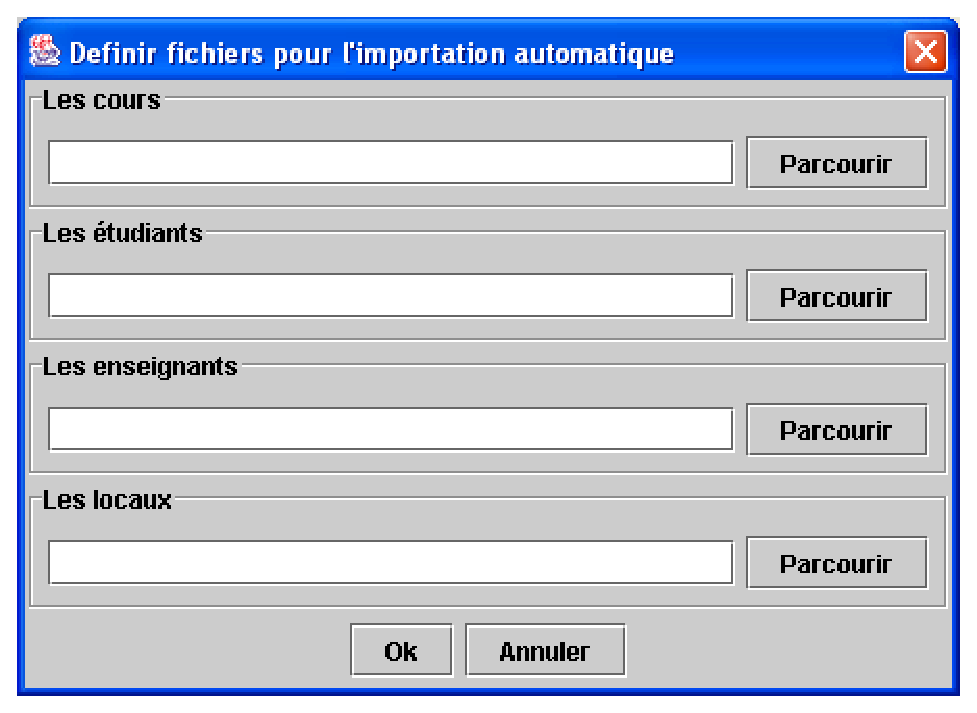
\includegraphics[width=2.5in]{UserManualInputs/images/autoimport.eps}
    \caption{D�finition des fichiers d'importation}\label{defautoimport}
  \end{center}
\end{figure}


    \item Aller au menu Fichier et s�lectionner le menu \textbf{\emph{Importer automatiquement}}. Une boite de dialogue apparaitra et vous permettra
\end{enumerate}    

\section{Horaire d'examen} 